\section{Sprint 3}

\subsection{Summary}

\begin{table}[H]
	\centering
	\begin{tabular}{ll}
		\toprule
		\multicolumn{2}{c}{\textbf{Sprint 3}}\\
		\midrule
		\textbf{Periode} & 16.03.2015 12:00 Uhr\textendash 30.03.2015 12:00 Uhr\\
		\textbf{Stunden Soll} & \SI{144}{\hour}\\
		\textbf{Stunden Plan} & \SI{145}{\hour} \\
		\textbf{Stunden Ist} & \SI{204.3}{\hour}\\
		\bottomrule
	\end{tabular}
\end{table}

\begin{figure}[H]
	\centering
	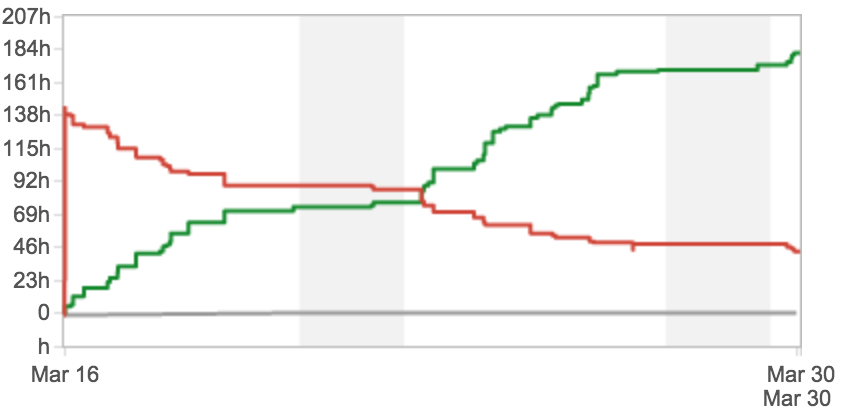
\includegraphics{fig/bd-sprint-3}
	\label{fig:pm:bd-sprint-3}
	\caption*{Burndown Chart Sprint 3}
\end{figure}

\subsection{Ziele}
Das Hauptziel dieses Sprints ist ein Fundament für restliche Applikation/Entwicklung zu schaffen. Es sollten diverse Dateiformate in eine geeignete Datenstruktur geladen werden um diese wiederum in andere Formate zu konvertieren bzw. ``formatieren'' zu können.

\begin{itemize}
	\item ``Plugin/Pluggable'' Interface für Daten Extractors/Parsers Transformers und Formatters
	\item Diverse Dateiformate einlesen und konvertieren können
	\item Authentifizierung
\end{itemize}

\subsection{Abgeschlossen}
Folgende High-level (ohne Subtasks) Jira Tasks wurden während Sprint 3 abgeschlossen. Ab dem nächsten Sprint werden zur besseren Übersicht alle ``Übrigen Aufwände'' sowie Sitzungen zusammengefasst. Eine Auswertung pro Person bleibt dennoch möglich.

\begin{table}[H]
\centering
\begin{tabular}{ll}
	\toprule
	\textbf{JIRA-Key} & \textbf{Summary}\\
	\midrule
DAT-49 & Refactoring Sprint 2\\
DAT-50 & Benutzerverwaltung/OAuth\\
DAT-51 & Liste der Dokumente\\
DAT-52 & Detailansicht Dokument\\
DAT-56 & Besseres Design/Layout\\
DAT-57 & Extractor/Transformer Interface bestimmten\\
DAT-64 & Projektmeeting Woche 5\\
DAT-65 & Projektmeeting Woche 6\\
DAT-66 & Organisation, Planung \& Kommunikation\\
DAT-69 & Übrige Aufwände Remo\\
DAT-70 & Übrige Aufwände Fabio\\
DAT-71 & Übrige Aufwände Christoph\\
	\bottomrule
\end{tabular}	
\end{table}

\subsection{Probleme}
Die Authentifizierung via OAuth hat aufgrund erstmaliger Einarbeitung in AngularJS mehr Zeit beansprucht als geplant.
